\label{sec:overview}
\begin{figure}
	\centering
		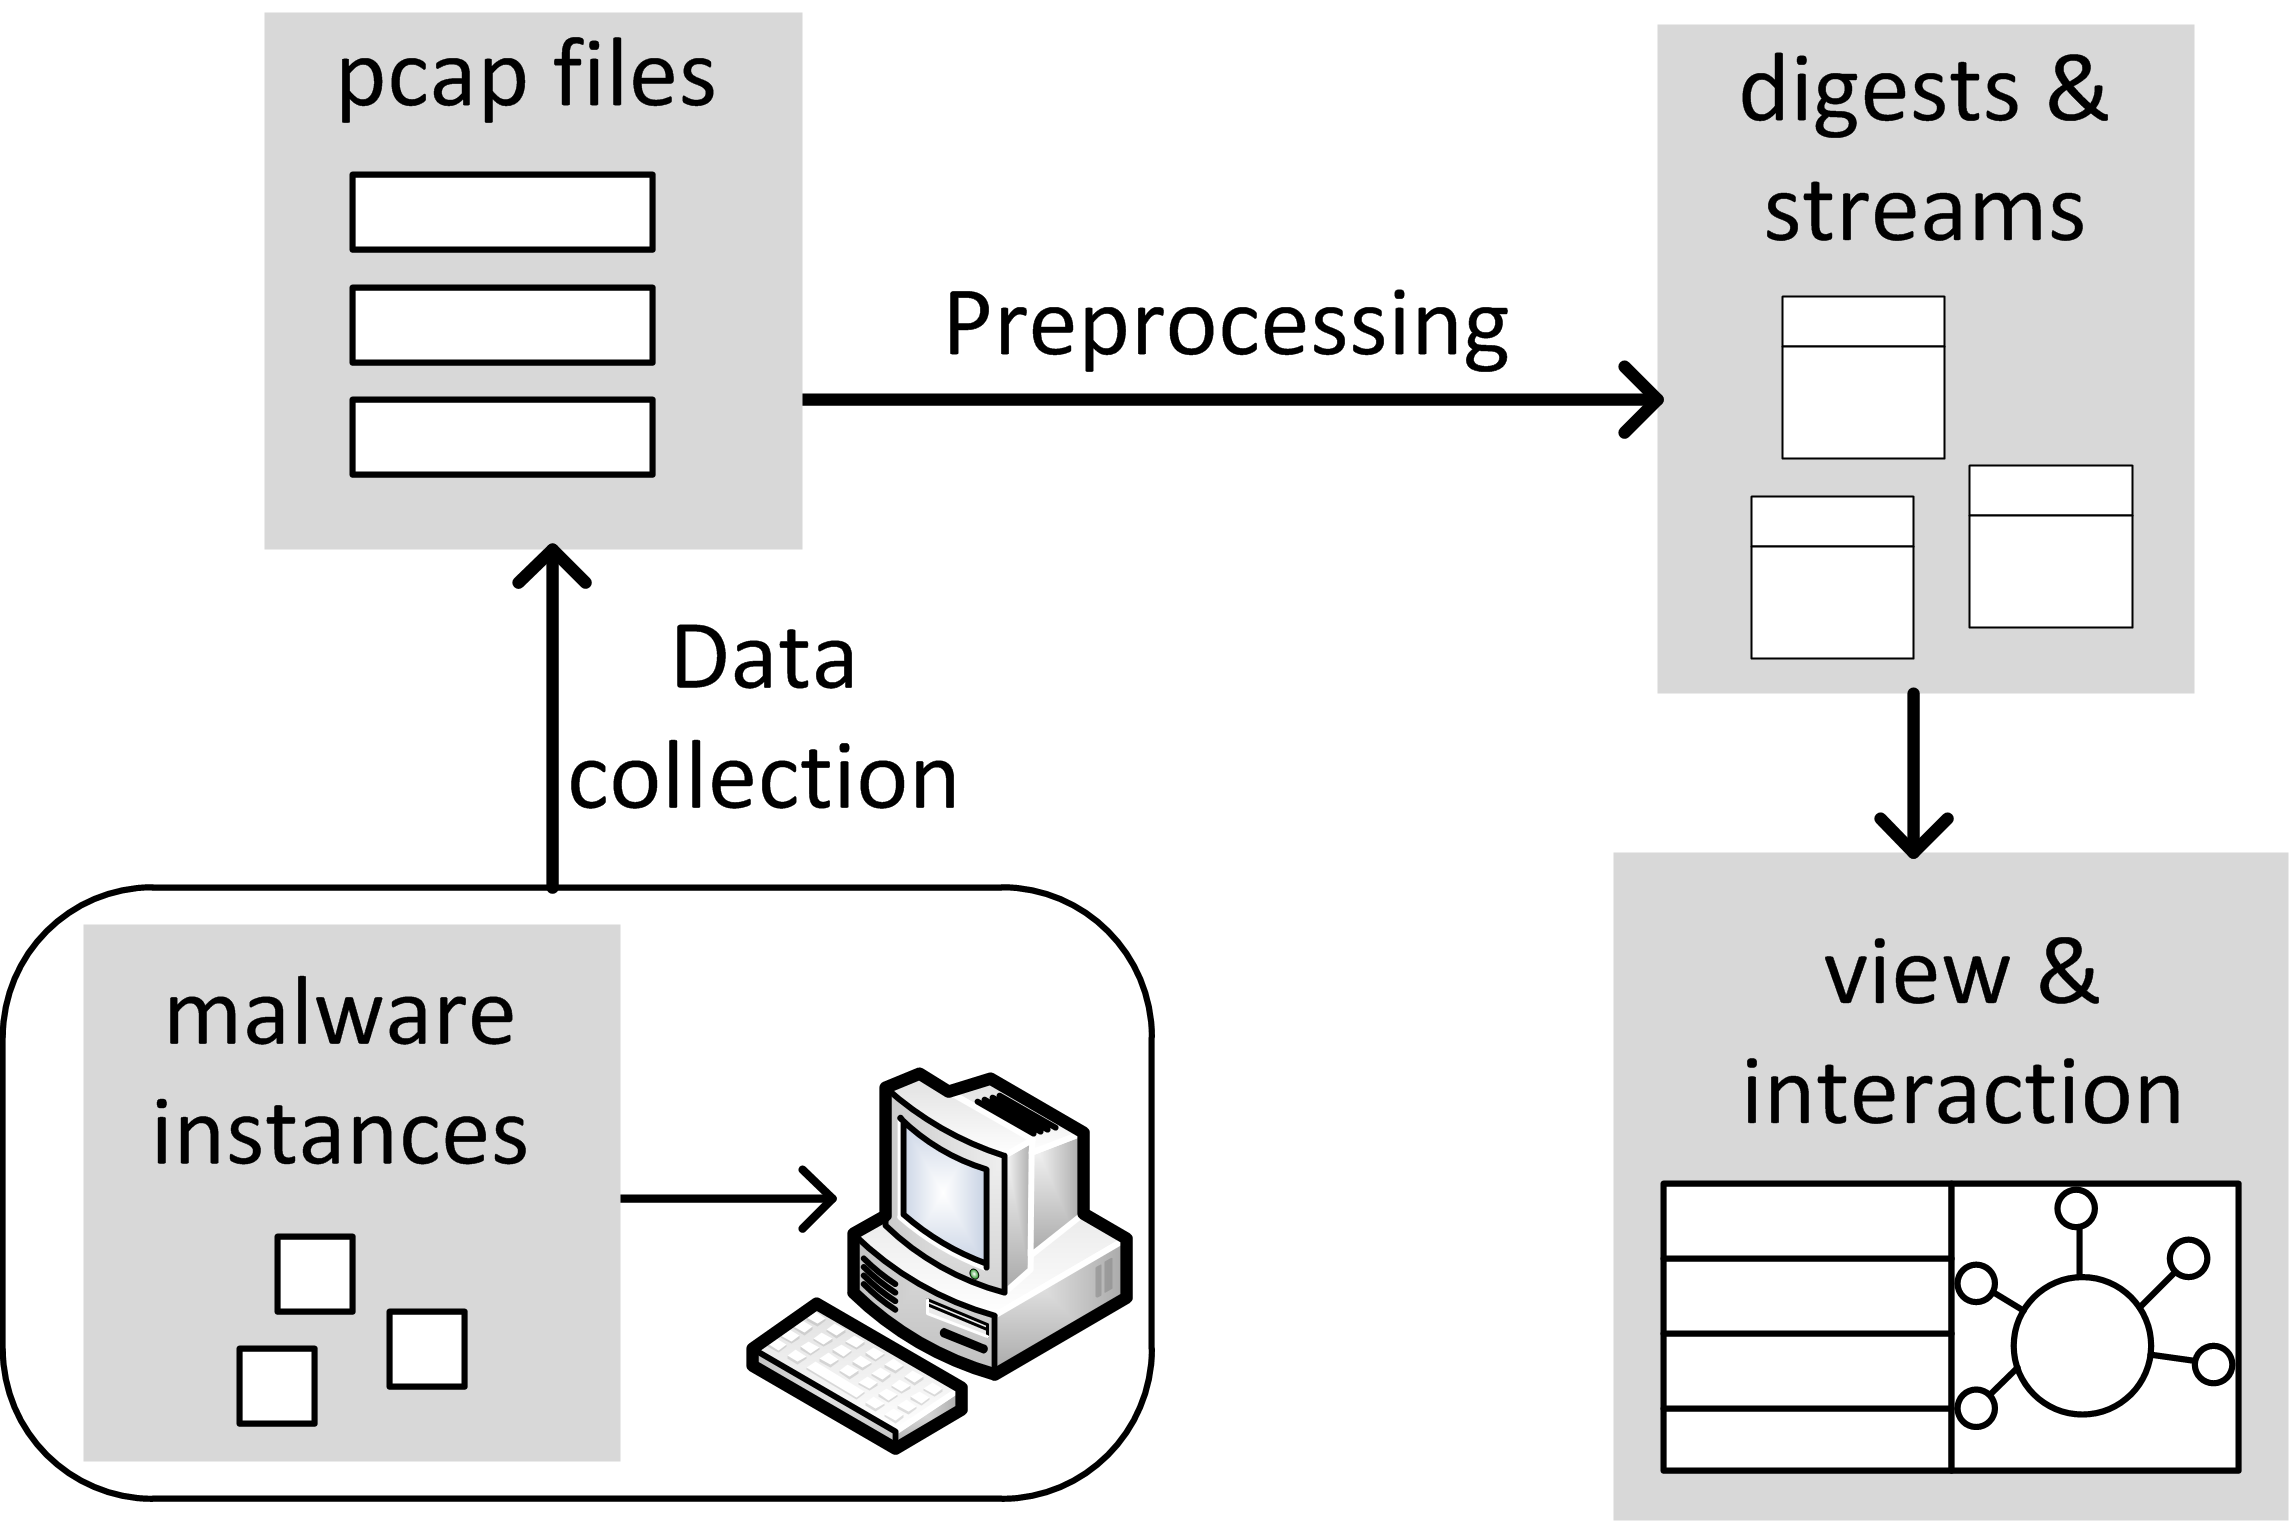
\includegraphics[width=\linewidth]{pics/Overview.png}
	\caption{The overview of our malware visual analytic system. The user-end view and interaction rely on three primary modules: data collection, preprocessing and visualization.}
		\label{fig:Overview}
\end{figure}

We show an overview of our malware visual analytic system in Fig.~\ref{fig:Overview}, complemented by the discussion of how malware network data are captured, processed and visualized in this section. As shown in the figure, the process consists of three primary modules: \emph{data collection}, \emph{preprocessing}, and \emph{visualization}. 

\textbf{Data sources.} First we gather a subset of recent malware corpus. Samples were collected from honeypots, mail filters, proxy monitors, web crawling, file sharing networks, etc. The testing set consisted of 200 MD5 unique malware instances. We analyze the malware binaries by executing them for three minutes in a virtualized dynamic malware analysis system, similar to previously described systems~(\cite{Bayer06}~\cite{Willems:2007}~\cite{Dinaburg08}), and record all the network traffic into packet traces as pcap files\footnote{\url{www.tcpdump.org}}. Precautions were taken to prevent the executing malware from acting maliciously; specifically, we redirected sent email to a spam trap, blocked connections to ports commonly used by exploits and blocked traffic to other local machines.

\textbf{Preprocessing.} Then, we parse pcap files into a set of appropriately formatted documents which we refer to as malware entities. Each entity is of the form 

\verb+<Digest D | ArrayList<Stream> S>+

The structure \emph{Digest} consists of MD5, total number of packets, total size of transmission~(including overhead from the headers), total number of streams, and duration. The list of streams are extracted from the protocol information in a pcap file. Specifically, each stream is a entity itself with heterogeneous attribute value types that include host~(IP or domain name), protocol~(DNS or TCP), number of packets~($n$), size of transmission~($z$), relative start time~($s$), duration~($t$), and validity. A DNS stream is defined as a DNS request and its corresponding response and a TCP stream begins with a 3-way TCP handshake and concludes with successful or unsuccessful termination.
 
\textbf{Visualization.} The visualization module generates table views and cell views. Given a set of entity records, the user browses the table of digests and select one or several target entities. Then the application generates a stream table and a cell view for each selected entity. Our attributes mapping and layout algorithms run in real-time for most of the malware entities supplied. In a typical visual analysis scenario, the user interacts with the cell view by selecting a 'cilium' that represent a stream of interest. Details of the stream, such as its host ip and country name, are displayed at the disk panel located at the center of the cell view. The user can adjust the layout parameters for the circular timeline interactively so as to improve the clarity of the set of cilia~(Sec.~\ref{sec:timeline}).
      


               

